\subsection{GP Results}



\begin{figure*}[htp]
  \centering
  \subfloat[]{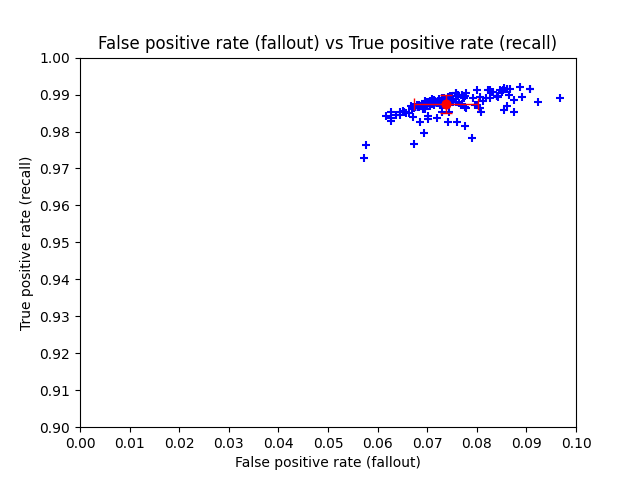
\includegraphics[scale=0.5]{figs/FPR_TPR_NS_MS1_PP.png}}\quad
  \subfloat[]{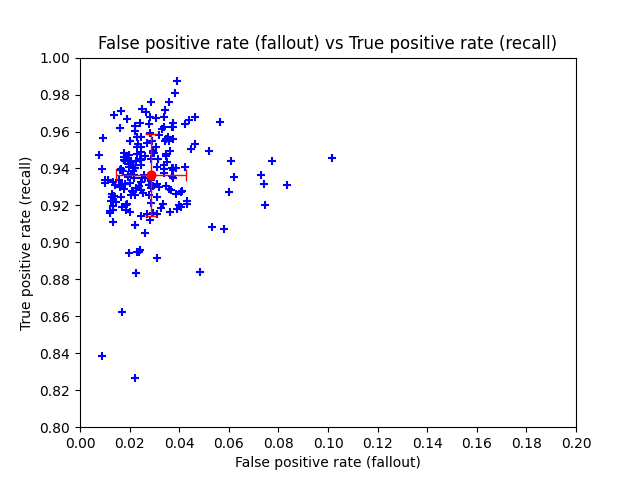
\includegraphics[scale=0.5]{figs/FPR_TPR_EMB_MS1_PP.png}}
  \caption{The plot on the left is a FPR (False Positive Rate) vs (True Positive Rate) plot for all 200 winning expressions for hasNS classification on MS1-PP EoS. The red dot is the average of TPR and FPR of the expressions and the vetricle and horizontal spread are the one sigma values for TPR and FPR respectively. The plot on the right is similar but for hasRemnant classification.  }
  \label{fig:FPR_TPR}
\end{figure*}

There as some caveats to this calculation. Given a finite testing set, we cannot fully compute the entire parameter space (201 x 201 cases) of the probability since there are some cases which are highly unlikely to occur, like $p(hasNS | XNS=0 \cap XREM=200)$. Also, our probability computations might also suffer due to the finite testing set size. The resulting probability distribution is highly rugged and \textcolor{red}{discontinuous or incomplete}. Hence, in order to span the entire parameter space of the probability, we use gasussian process regression (GPR). 

\textbf{Gaussian Process Regression:} We implement GPR using a python package gpytorch \cite{gpytorch}. Using the Rational Quadratic(RQ) kernel of the gpytorch , we compute a smooth probability distribution over all possible combination of XREM and XNS as shown in Fig \ref{fig:probability}. The selection of the parameters for GPR was motivated by two major factors. The first being that probability had to be confined between interval [0,1] and the case $P(hasNS)$ or $P(hasRemnant) ~ 1$ when $XNS$ and $XREM$ approaches maximum number of trees.The second being the condition $p(hasNS| XREM \cap XNS) \geq p(hasRemnant| XREM \cap XNS)$. After multiple trials, we found that using 200 winning expression and using length scale interval [$1X10^{-5}, 1X10^{5}$] and alpha parameter interval [$1X10^{-5}, 10$] for GPR, we can obtain desired probability distribution.

\begin{figure*}[htp]
  \centering
  \subfloat[]{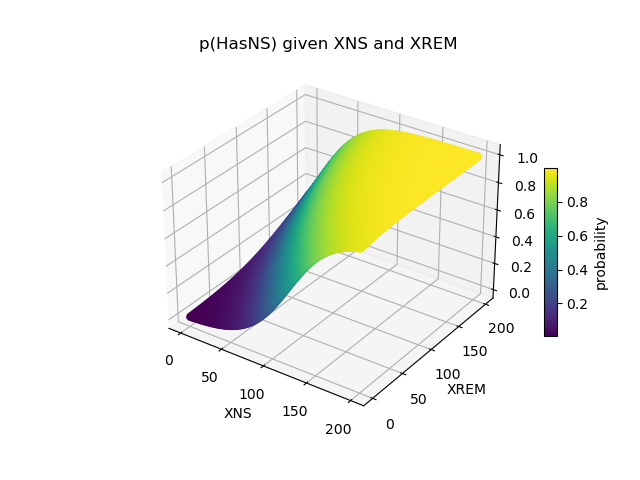
\includegraphics[scale=0.5]{figs/Probability_NS_MS1_PP.png}}\quad
  \subfloat[]{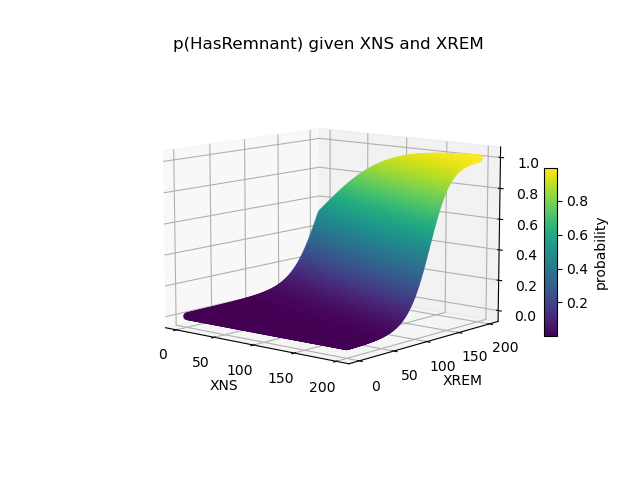
\includegraphics[scale=0.5]{figs/Probability_EMB_MS1_PP.png}}
  \caption{The plot on the left is the probability distrbution of equation \ref{eq:1} after GPR implementation for MS1-PP EoS.  The plot on the right is a similar plot of equation \ref{eq:2}  }
  \label{fig:probability}
\end{figure*}

Using this probablity, we make the ROC curve using the testing set for all the EoS as shown in \ref{fig:ROC}. 

\begin{figure*}[htp]
  \centering
  \subfloat[]{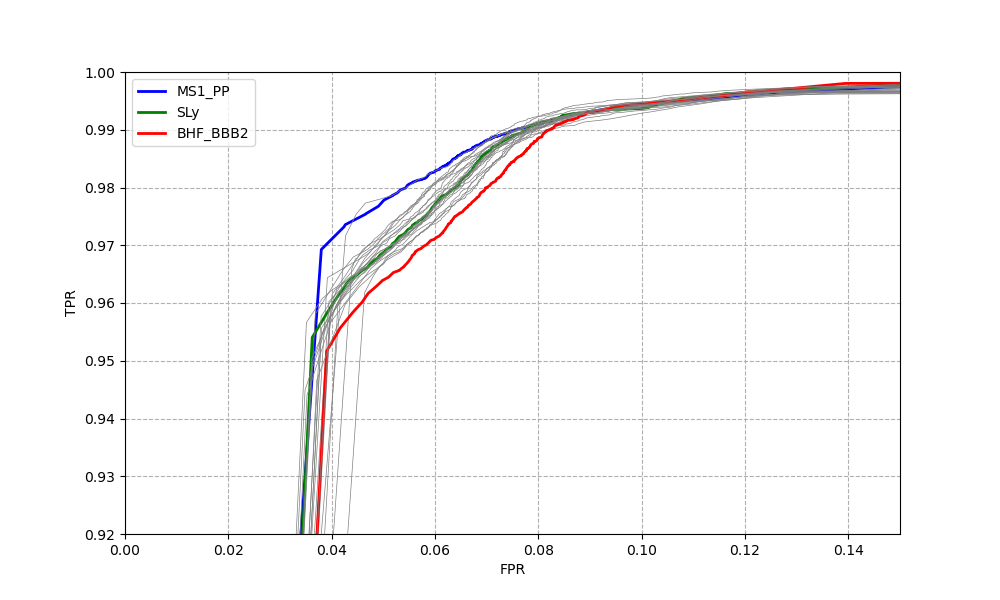
\includegraphics[scale=0.30]{figs/ROC_NS.png}}\quad
  \subfloat[]{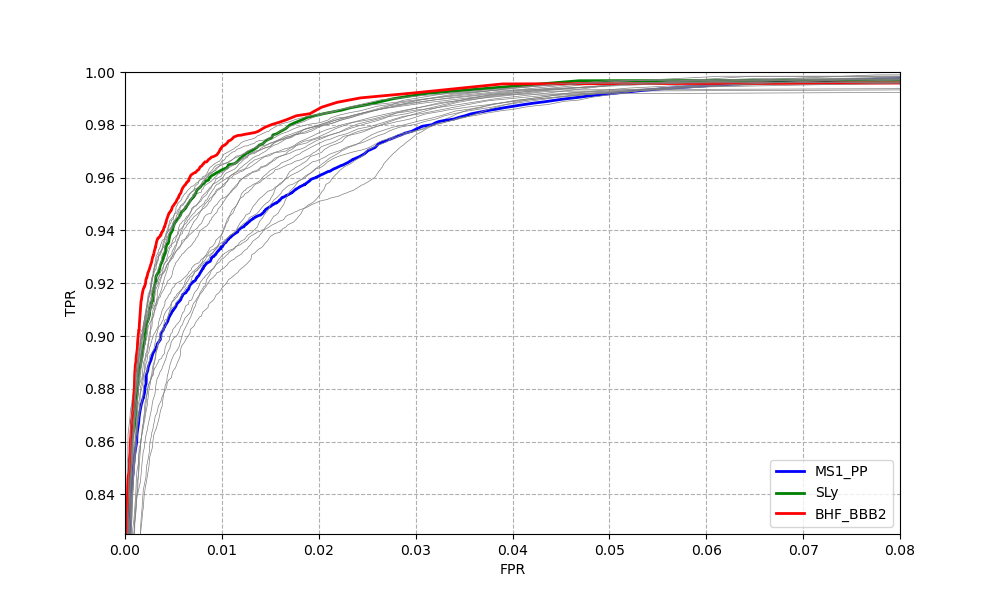
\includegraphics[scale=0.30]{figs/ROC_EMB.png}}
  \caption{The plot on the left is the ROC curve for hasHS label evaluated on the testing set whereas the plot in the right is for hasRemnant for all 23 EoS. }
  \label{fig:ROC}
\end{figure*}
